%%
%% This is file `sample-sigconf.tex',
%% generated with the docstrip utility.
%%
%% The original source files were:
%%
%% samples.dtx  (with options: `sigconf')
%% 
%% IMPORTANT NOTICE:
%% 
%% For the copyright see the source file.
%% 
%% Any modified versions of this file must be renamed
%% with new filenames distinct from sample-sigconf.tex.
%% 
%% For distribution of the original source see the terms
%% for copying and modification in the file samples.dtx.
%% 
%% This generated file may be distributed as long as the
%% original source files, as listed above, are part of the
%% same distribution. (The sources need not necessarily be
%% in the same archive or directory.)
%%
%%
%% Commands for TeXCount
%TC:macro \cite [option:text,text]
%TC:macro \citep [option:text,text]
%TC:macro \citet [option:text,text]
%TC:envir table 0 1
%TC:envir table* 0 1
%TC:envir tabular [ignore] word
%TC:envir displaymath 0 word
%TC:envir math 0 word
%TC:envir comment 0 0
%%
%%
%% The first command in your LaTeX source must be the \documentclass
%% command.
%%
%% For submission and review of your manuscript please change the
%% command to \documentclass[manuscript, screen, review]{acmart}.
%%
%% When submitting camera ready or to TAPS, please change the command
%% to \documentclass[sigconf]{acmart} or whichever template is required
%% for your publication.
%%
%%
\documentclass[sigconf,anonymous, review]{acmart}

\usepackage{dsfont}
\usepackage{array}
\usepackage{makecell}
\usepackage{xeCJK}
\setCJKmainfont[BoldFont=STKaiti, ItalicFont=STKaiti]{STKaiti-Regular}


%%
%% \BibTeX command to typeset BibTeX logo in the docs
\AtBeginDocument{%
	\providecommand\BibTeX{{%
			Bib\TeX}}}

%% Rights management information.  This information is sent to you
%% when you complete the rights form.  These commands have SAMPLE
%% values in them; it is your responsibility as an author to replace
%% the commands and values with those provided to you when you
%% complete the rights form.
\setcopyright{acmcopyright}
\copyrightyear{2018}
\acmYear{2018}
\acmDOI{XXXXXXX.XXXXXXX}


%% These commands are for a PROCEEDINGS abstract or paper.
\acmConference[Conference acronym 'XX]{Make sure to enter the correct
	conference title from your rights confirmation emai}{June 03--05,
	2018}{Woodstock, NY}
%%
%%  Uncomment \acmBooktitle if the title of the proceedings is different
%%  from ``Proceedings of ...''!
%%
%%\acmBooktitle{Woodstock '18: ACM Symposium on Neural Gaze Detection,
%%  June 03--05, 2018, Woodstock, NY}
\acmPrice{15.00}
\acmISBN{978-1-4503-XXXX-X/18/06}


%%
%% Submission ID.
%% Use this when submitting an article to a sponsored event. You'll
%% receive a unique submission ID from the organizers
%% of the event, and this ID should be used as the parameter to this command.
%%\acmSubmissionID{123-A56-BU3}

%%
%% For managing citations, it is recommended to use bibliography
%% files in BibTeX format.
%%
%% You can then either use BibTeX with the ACM-Reference-Format style,
%% or BibLaTeX with the acmnumeric or acmauthoryear sytles, that include
%% support for advanced citation of software artefact from the
%% biblatex-software package, also separately available on CTAN.
%%
%% Look at the sample-*-biblatex.tex files for templates showcasing
%% the biblatex styles.
%%

%%
%% The majority of ACM publications use numbered citations and
%% references.  The command \citestyle{authoryear} switches to the
%% "author year" style.
%%
%% If you are preparing content for an event
%% sponsored by ACM SIGGRAPH, you must use the "author year" style of
%% citations and references.
%% Uncommenting
%% the next command will enable that style.
%%\citestyle{acmauthoryear}


\newcommand{\1}[1]{\mathds{1}\left[#1\right]}

\newcommand{\secref}[1]{Section \ref{#1}}
\newcommand{\figref}[1]{Figure \ref{#1}}
\newcommand{\eqnref}[1]{Eq. (\ref{#1})}
\newcommand{\exref}[1]{Example \ref{#1}}
\newcommand{\algoref}[1]{Algorithm \ref{#1}}
\newcommand{\tabref}[1]{Table \ref{#1}}
\newcommand{\socvec}{SocVec}
\newcommand{\argmin}{\operatornamewithlimits{argmin}}
\newcommand{\argmax}{\operatornamewithlimits{argmax}}
\newtheorem{example}{Example}
\newtheorem{lemma}{Lemma}
\newtheorem{definition}{Definition}
\newcommand{\cut}[1]{}
\newcommand{\ZY}[1]{\textcolor{red}{Zhiyi: #1}}

%%
%% end of the preamble, start of the body of the document source.
\begin{document}
	
	%%
	%% The "title" command has an optional parameter,
	%% allowing the author to define a "short title" to be used in page headers.
	\title{Towards Domain Knowledge Enhanced Pre-training with ChatGPT}
	
	%%
	%% The "author" command and its associated commands are used to define
	%% the authors and their affiliations.
	%% Of note is the shared affiliation of the first two authors, and the
	%% "authornote" and "authornotemark" commands
	%% used to denote shared contribution to the research.
	\author{Ben Trovato}
	\authornote{Both authors contributed equally to this research.}
	\email{trovato@corporation.com}
	\orcid{1234-5678-9012}
	\author{G.K.M. Tobin}
	\authornotemark[1]
	\email{webmaster@marysville-ohio.com}
	\affiliation{%
		\institution{Institute for Clarity in Documentation}
		\streetaddress{P.O. Box 1212}
		\city{Dublin}
		\state{Ohio}
		\country{USA}
		\postcode{43017-6221}
	}
	
	\author{Lars Th{\o}rv{\"a}ld}
	\affiliation{%
		\institution{The Th{\o}rv{\"a}ld Group}
		\streetaddress{1 Th{\o}rv{\"a}ld Circle}
		\city{Hekla}
		\country{Iceland}}
	\email{larst@affiliation.org}
	
	\author{Valerie B\'eranger}
	\affiliation{%
		\institution{Inria Paris-Rocquencourt}
		\city{Rocquencourt}
		\country{France}
	}
	
	\author{Aparna Patel}
	\affiliation{%
		\institution{Rajiv Gandhi University}
		\streetaddress{Rono-Hills}
		\city{Doimukh}
		\state{Arunachal Pradesh}
		\country{India}}
	
	\author{Huifen Chan}
	\affiliation{%
		\institution{Tsinghua University}
		\streetaddress{30 Shuangqing Rd}
		\city{Haidian Qu}
		\state{Beijing Shi}
		\country{China}}
	
	\author{Charles Palmer}
	\affiliation{%
		\institution{Palmer Research Laboratories}
		\streetaddress{8600 Datapoint Drive}
		\city{San Antonio}
		\state{Texas}
		\country{USA}
		\postcode{78229}}
	\email{cpalmer@prl.com}
	
	\author{John Smith}
	\affiliation{%
		\institution{The Th{\o}rv{\"a}ld Group}
		\streetaddress{1 Th{\o}rv{\"a}ld Circle}
		\city{Hekla}
		\country{Iceland}}
	\email{jsmith@affiliation.org}
	
	\author{Julius P. Kumquat}
	\affiliation{%
		\institution{The Kumquat Consortium}
		\city{New York}
		\country{USA}}
	\email{jpkumquat@consortium.net}
	
	
	%%
	%% By default, the full list of authors will be used in the page
	%% headers. Often, this list is too long, and will overlap
	%% other information printed in the page headers. This command allows
	%% the author to define a more concise list
	%% of authors' names for this purpose.
	\renewcommand{\shortauthors}{Trovato et al.}
	
	%%
	%% The abstract is a short summary of the work to be presented in the
	%% article.
	\begin{abstract}
		A clear and well-documented \LaTeX\ document is presented as an
		article formatted for publication by ACM in a conference proceedings
		or journal publication. Based on the ``acmart'' document class, this
		article presents and explains many of the common variations, as well
		as many of the formatting elements an author may use in the
		preparation of the documentation of their work.
	\end{abstract}
	
	%%
	%% The code below is generated by the tool at http://dl.acm.org/ccs.cfm.
	%% Please copy and paste the code instead of the example below.
	%%
	\begin{CCSXML}
		<ccs2012>
		<concept>
		<concept_id>00000000.0000000.0000000</concept_id>
		<concept_desc>Do Not Use This Code, Generate the Correct Terms for Your Paper</concept_desc>
		<concept_significance>500</concept_significance>
		</concept>
		<concept>
		<concept_id>00000000.00000000.00000000</concept_id>
		<concept_desc>Do Not Use This Code, Generate the Correct Terms for Your Paper</concept_desc>
		<concept_significance>300</concept_significance>
		</concept>
		<concept>
		<concept_id>00000000.00000000.00000000</concept_id>
		<concept_desc>Do Not Use This Code, Generate the Correct Terms for Your Paper</concept_desc>
		<concept_significance>100</concept_significance>
		</concept>
		<concept>
		<concept_id>00000000.00000000.00000000</concept_id>
		<concept_desc>Do Not Use This Code, Generate the Correct Terms for Your Paper</concept_desc>
		<concept_significance>100</concept_significance>
		</concept>
		</ccs2012>
	\end{CCSXML}
	
	\ccsdesc[500]{Do Not Use This Code~Generate the Correct Terms for Your Paper}
	\ccsdesc[300]{Do Not Use This Code~Generate the Correct Terms for Your Paper}
	\ccsdesc{Do Not Use This Code~Generate the Correct Terms for Your Paper}
	\ccsdesc[100]{Do Not Use This Code~Generate the Correct Terms for Your Paper}
	
	%%
	%% Keywords. The author(s) should pick words that accurately describe
	%% the work being presented. Separate the keywords with commas.
	\keywords{multi-span question answering, reading comprehension, chinese datasets, joint learning, neural networks}
	%% A "teaser" image appears between the author and affiliation
	%% information and the body of the document, and typically spans the
	%% page.
%	\begin{teaserfigure}
%		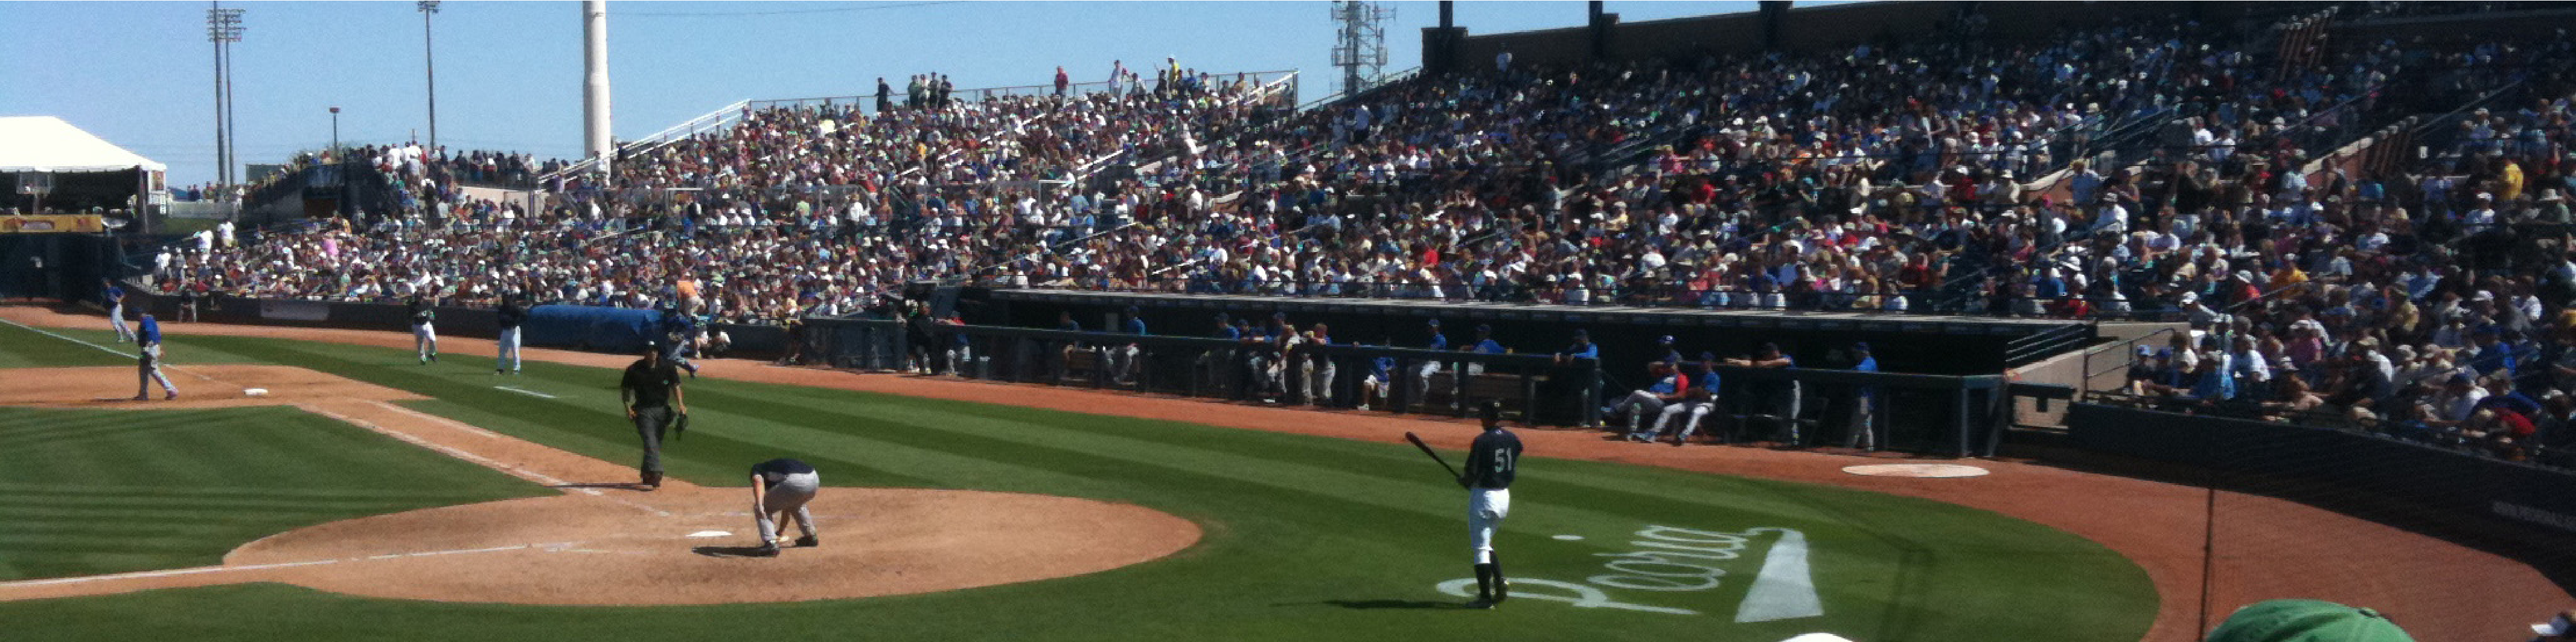
\includegraphics[width=\textwidth]{sampleteaser}
%		\caption{Seattle Mariners at Spring Training, 2010.}
%		\Description{Enjoying the baseball game from the third-base
%			seats. Ichiro Suzuki preparing to bat.}
%		\label{fig:teaser}
%	\end{teaserfigure}
	
%	\received{20 February 2007}
%	\received[revised]{12 March 2009}
%	\received[accepted]{5 June 2009}
	
	%%
	%% This command processes the author and affiliation and title
	%% information and builds the first part of the formatted document.
	\maketitle
	
	\section{Introduction}
\label{sec:introduction}
	\section{Preliminary}
\label{sec:preliminary}
	\section{Experiments}
\label{sec:experiments}
	\section{Related Work}
\label{sec:related}
	\section{Conclusion}
\label{sec:conclusion}
	At last, let's cite a paper~\cite[Luo]{Abril07}.


%%
%% The acknowledgments section is defined using the "acks" environment
%% (and NOT an unnumbered section). This ensures the proper
%% identification of the section in the article metadata, and the
%% consistent spelling of the heading.
%\begin{acks}
%	To Robert, for the bagels and explaining CMYK and color spaces.
%\end{acks}

%%
%% The next two lines define the bibliography style to be used, and
%% the bibliography file.
\bibliographystyle{ACM-Reference-Format}
\bibliography{refs}


%%
%% If your work has an appendix, this is the place to put it.
%\appendix
%
%\section{Research Methods}
%
%\subsection{Part One}
%
%Lorem ipsum dolor sit amet, consectetur adipiscing elit. Morbi
%malesuada, quam in pulvinar varius, metus nunc fermentum urna, id
%sollicitudin purus odio sit amet enim. Aliquam ullamcorper eu ipsum
%vel mollis. Curabitur quis dictum nisl. Phasellus vel semper risus, et
%lacinia dolor. Integer ultricies commodo sem nec semper.
%
%\subsection{Part Two}
%
%Etiam commodo feugiat nisl pulvinar pellentesque. Etiam auctor sodales
%ligula, non varius nibh pulvinar semper. Suspendisse nec lectus non
%ipsum convallis congue hendrerit vitae sapien. Donec at laoreet
%eros. Vivamus non purus placerat, scelerisque diam eu, cursus
%ante. Etiam aliquam tortor auctor efficitur mattis.
%
%\section{Online Resources}
%
%Nam id fermentum dui. Suspendisse sagittis tortor a nulla mollis, in
%pulvinar ex pretium. Sed interdum orci quis metus euismod, et sagittis
%enim maximus. Vestibulum gravida massa ut felis suscipit
%congue. Quisque mattis elit a risus ultrices commodo venenatis eget
%dui. Etiam sagittis eleifend elementum.
%
%Nam interdum magna at lectus dignissim, ac dignissim lorem
%rhoncus. Maecenas eu arcu ac neque placerat aliquam. Nunc pulvinar
%massa et mattis lacinia.

\end{document}
\endinput
%%
%% End of file `sample-sigconf.tex'.
